\documentclass[aps,prb,twocolumn,superscriptaddress]{revtex4-2}
\usepackage{graphicx}  % Required for inserting images
\usepackage{hyperref}  % Required for clickable links
\usepackage{wrapfig}
\usepackage{amsmath}

\renewcommand{\thefigure}{\arabic{figure}}

\hypersetup{
    colorlinks=true,
    linkcolor=blue,
    filecolor=magenta,      
    urlcolor=cyan,
}

\begin{document}

\title{Advancements in X-Ray Diffraction and X-Ray Free-Electron Lasers}

\author{Simon Lavoie}
\affiliation{Department of Physics, McGill University}
\date{February 2025}

\begin{abstract}
Due to their nanometer-scale wavelengths, X-rays are well-suited for probing
atomic-scale structures.  This paper discusses advancements in X-ray diffraction
(XRD) and the impact of improved X-ray sources, including synchrotrons and X-ray
free-electron lasers (XFELs), on structural studies in physics, chemistry, and
biology. Topics include the historical context of XRD, Bragg's law, experimental
techniques, and modern computational analysis methods such as Fourier transform
analysis and Rietveld refinement.  Challenges in data acquisition and recent
technological developments will also be explored.
\end{abstract}

\maketitle

\section*{Contents}
\begin{itemize}
    \item \hyperref[sec:intro]{Introduction}
    \item \hyperref[sec:theory]{Theoretical Framework}
    \item \hyperref[sec:experiment]{Experimental Methods}
    \item \hyperref[sec:data]{Data Acquisition and Analysis}
    \item \hyperref[sec:challenges]{Challenges and Future Prospects}
\end{itemize}

\section{Introduction} \label{sec:intro}
X-ray diffraction (XRD) has been instrumental in elucidating atomic structures
since its experimental validation in 1912.  With the advent of synchrotrons and
XFELs, the technique has undergone significant refinement, enabling
time-resolved imaging and single-particle studies.

\section{Theoretical Framework} \label{sec:theory}
\subsection{Bragg's Law}
Shortly after Röntgen's discovery of X-rays, Max von Laue suggested that X-rays
could be diffracted by crystals, which Friedrich and Knipping experimentally
confirmed in 1912. The underlying principle was formalized by W. H. Bragg and W.
L. Bragg through:
\begin{equation}\label{eq:bragg}
  2d\sin\theta = n\lambda,
\end{equation}
where $d$ is the regular spacing between the atoms, $\theta$ the angle of
incidence, $n$ an integer, and $\lambda$ the X-ray wavelength \cite{Bragg1913}.
As an X-ray beam incident upon a crystal interacts with the electrons of the
lattice's atoms, it is scattered spherically in all directions. The scattered
X-rays from adjacent atoms interfere constructively and destructively, producing
a diffracted beam. The condition for constructive interference is given by Eq.
\ref{eq:bragg}. That is, when the path difference between two adjacent rays
($2d\sin\theta$) is an integer multiple of the wavelength, the waves will
superimpose in phase, leading to peaks in the diffracted intensity. This
phenomenon is illustrated in Fig. \ref{fig:Laue}.

% BRAGG DIFFRACTION FIGURE
\begin{figure}[!h]
    \centering
    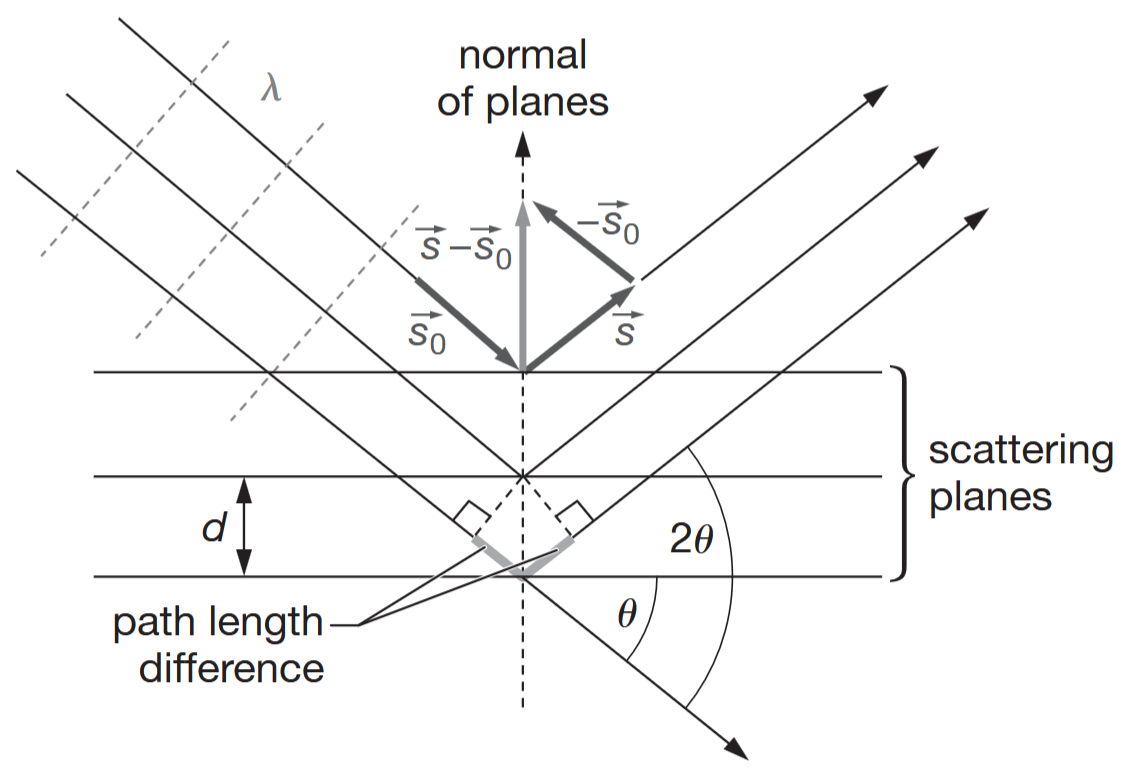
\includegraphics[width=0.9\linewidth]{Figures/Bragg_diffraction_2.svg.png}
    \caption{Geometry of a beam with angle of incidence $\theta$ approaching from the left
    into a symmetrical arrangement of atoms forming the lattice of a crystal \cite{Girolami}. }
    \label{fig:Bragg}
\end{figure}

% LAUE DIFFRACTION PATTERN
\begin{figure}[h]
    \centering
    \includegraphics[width=0.9\linewidth]{Figures/Interferenz-Erscheinungen_bei_Röntgenstrahlen_Tafel_II_Fig._5.jpg}
    \caption{X-ray diffraction pattern of a copper sulfate crystal from
    Friedrich and Knipping's 1912 paper \cite{vonLaue1912}.} \label{fig:Laue}
\end{figure}

\subsection{The Structure of Crystals}
The theory of crystals and how they are structured is essential to understanding
X-ray diffraction. Crystals are regular arrangements of atoms in three
dimensions, exhibiting translational symmetry. The discrete points at which the
atoms of a crystal are located can be described mathematically by 
\begin{equation}\label{eq:lattice}
    \mathbf{R} = n_1\mathbf{a}_1 + n_2\mathbf{a}_2 + n_3\mathbf{a}_3,   
\end{equation}
where $\mathbf{a}_1$, $\mathbf{a}_2$, and $\mathbf{a}_3$ are the primitive
vectors of the lattice and $n_1$, $n_2$, and $n_3$ are integers. This infinite
set of points defined by Eq. \ref{eq:lattice} forms a Bravais lattice, and the
parallelepiped comprised of these primitive vectors is called the unit cell. The
constraint that crystals exhibit translational symmetry and repeat periodically
in space leads to the classification of Bravais lattices into 14 distinct types
\cite{lattice_types}.  These lattices can be further categorized into seven
crystal systems based on the symmetry of the unit cell. The seven crystal
systems are cubic, tetragonal, orthorhombic, hexagonal, rhombohedral,
monoclinic, and triclinic. The concept of a reciprocal lattice, which is
especially useful in X-ray diffraction, is defined as the set of all wave
vectors $\mathbf{k}$ that yield plane waves with the periodicity of the Bravais
lattice \cite{Ashcroft}.  The reciprocal lattice itself is spanned by three
primitive vectors $\mathbf{b}_1$, $\mathbf{b}_2$, and $\mathbf{b}_3$ which can
be generated from the lattice's primitive vectors via:

\begin{equation}\label{eq:reciprocal}
    \mathbf{b_i} = 2\pi \frac{\mathbf{a}_j \times \mathbf{a}_k}
    {\mathbf{a_i} \cdot (\mathbf{a}_j \times \mathbf{a}_k)},
\end{equation}

For any cyclic permutation of ${i,j,k} = {1, 2, 3}$. The triple scalar product
in the denominator is physically interpreted as the volume of the unit cell. The
factor of $2\pi$ ensures that the reciprocal lattice vectors are properly scaled
so that plane waves match the periodicity of the crystal. The reciprocal lattice
vector is then defined as:

\begin{equation}\label{eq:reciprocal_vector}
    \mathbf{G} = h\mathbf{b}_1 + k\mathbf{b}_2 + l\mathbf{b}_3,
\end{equation}

where $h$, $k$, and $l$ are integers, commonly known as the Miller indices.
$\mathbf{G}$ is perpendicular to the family of planes indexed by $(hkl)$, these
being the planes that diffract the incident X-rays.  The inter-planar
spacing $d$ for a cubic crystal, for example,
is given by:

\begin{equation}\label{eq:interplanar}
    d = \frac{a}{\sqrt{h^2 + k^2 + l^2}},
\end{equation}

where $a$ is the lattice parameter, which represents the length of the unit
cell's sides.  For a cubic crystal, we have $a = |\textbf{a}_1| = |\textbf{a}_2|
= |\textbf{a}_3|$.  For other crystal systems (e.g., tetragonal, orthorhombic),
the interplanar spacing depends on a more general relation between the Miller
indices, the lattice parameters, and the metric tensor of the crystal system
\cite{Liu2020}.





\section{Experimental Methods} \label{sec:experiment}
\subsection{X-ray Sources}
Modern XRD experiments use high-brilliance sources such as synchrotrons and
XFELs to generate X-rays. X-ray sources are characterised by their brilliance,
which is the ratio of the intensity (photons per second) of the beam to its
spatial coherence, which is proportional to the product of the size
$(\text{m}^2)$, bandwidth and angular divergence of the beam.  The difference in
brilliance between XFELs and synchrotrons is drastic, with XFELs exhibiting
higher brilliance by several orders of magnitude due to their high peak power
and short pulse duration \cite{Baillet2014}. A comparison of the avberage
brilliance of XFEL and synchrotron facilities is shown in Fig.
\ref{fig:brilliance}.

\begin{figure}[h]
    \centering
    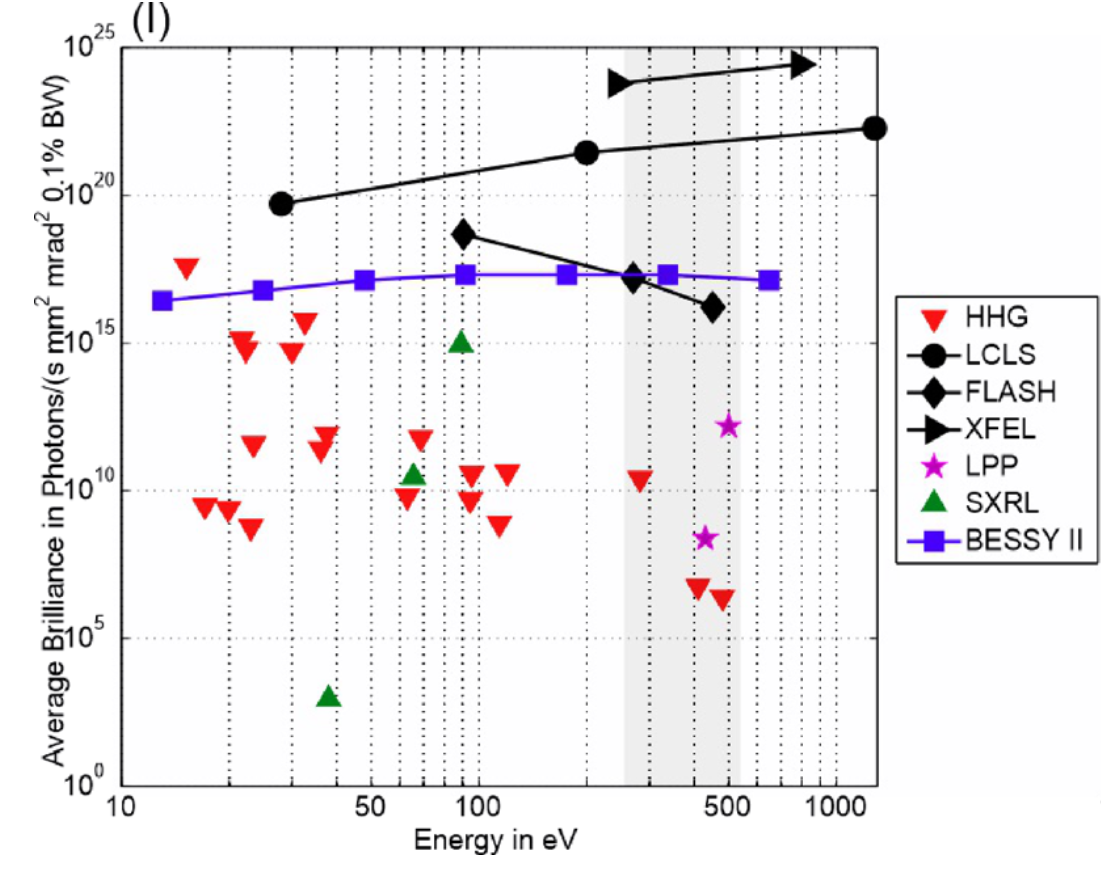
\includegraphics[width=0.9\linewidth]{Figures/XRaySourceBrilliance.png}
    \caption{Comparison of brilliance versus energy between X-ray user
        facilities on a log-log scale. \cite{Brilliance}. LCLS, FLASH and
        European XFEL (simply labelled XFEL) are XFELs, BESSY II is a
        synchrotron, and the others are High Harmonic Generation (HHG), Soft
        X-Ray Laser (SXRL) and Laser Produced Plasma (LPP) facilities.}
    \label{fig:brilliance}
\end{figure}

\begin{figure}[h]
    \centering
    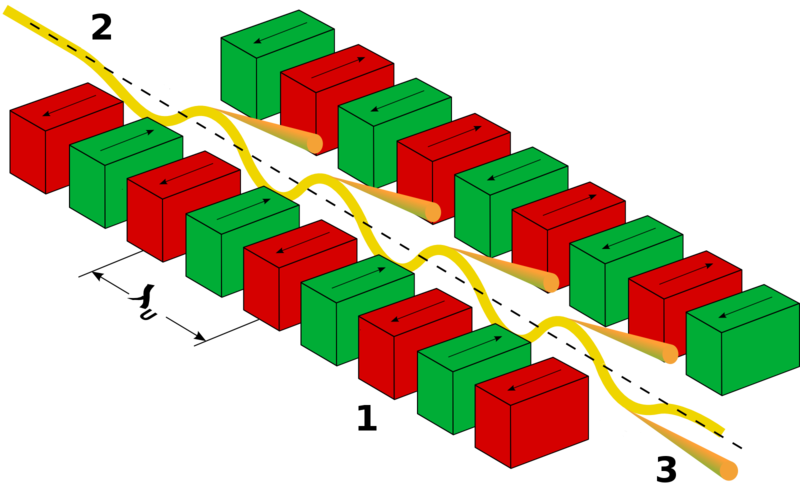
\includegraphics[width=0.9\linewidth]{Figures/800px-Undulator.png}
    \caption{Undulator schematic. Pictured are (1) two rows of adjacent magnets 
        of opposing polarities with spacing $\lambda_u/2$, (2) incident beam of
        electrons and (3) emitted radiation.}
    \label{fig:Undulator}
\end{figure}

These sources operate in a similar manner, accelerating
electrons to relativistic speeds before channeling them through undulators to
produce X-rays. Undulators, as can be seen in fig \ref{fig:Undulator}, are 
arrays of magnets of periodically alternating polarities. As an electron enters
this array at velocity $\textbf{u} \approx c$, it undergoes synchrotron 
radiation due to the acceleration caused by the sinusoidal magnetic field. In
the electron's centre of mass frame, where the undulator approaches at speed
$-\textbf{u}$, the undulator transverse $\textbf{B}$ field becomes the
combination of a transverse $\textbf{B}$ field and a transverse $\textbf{E}$
field via the Lorentz boosts:
\begin{align}
\mathbf{E}'_{\parallel} &= \mathbf{E}_{\parallel}, \quad \mathbf{B}'_{\parallel} = \mathbf{B}_{\parallel} \\
\mathbf{E}'_{\perp} &= \gamma (\mathbf{E}_{\perp} - u \mathbf{B}_{\perp}) \\
\mathbf{B}'_{\perp} &= \gamma \left( \mathbf{B}_{\perp} + \frac{u}{c^2} \mathbf{E}_{\perp} \right)
\end{align}
where $\gamma = \frac{1}{\sqrt{1 - v^2/c^2}}$ . Since the undulator field in
the lab frame is purely magnetic ($\textbf{E} = 0$), the transverse field in
the electron's rest frame simplifies to $\mathbf{E}'_{\perp} = - \gamma u
\mathbf{B}_{\perp}$. In essence, the system looks like an electromagnetic wave
approaching the electron, which in-turn causes the electron to radiate photons
of equal wavelength. This wavelength is given by the undulator period
$\lambda_u$ corrected for length contractions ($\lambda = \lambda_u/\gamma$).
However, the transverse velocity $\textbf{u}_{\perp}$ induced by the undulator
field slightly modifies the electron’s velocity components. Since the Lorentz
force cannot perform work, the total kinetic energy remains unchanged, but
$\textbf{u}_{\perp}$ reduces the electron’s longitudinal velocity to values
below $\textbf{u}$. It can therefore be shown that the wavelength measured in 
the lab frame becomes

\begin{equation}\label{equation: XFEL wl}
    \lambda = \frac{\lambda_u}{2\gamma^2}\left(1 + \frac{K^2}{2} \right)
\end{equation}

where,

\begin{equation}
    K = \frac{eB_0\lambda_u}{2\pi m_e c}.
\end{equation}
is known as the deflection parameter and is equal to the maximum angular
excursion of the beam in units of $1/\gamma$. Any device having $K < 1$ is
known as an undulator, while one with $K \gg 1$ is called a wiggler
\cite{Properties of Undulator Radiation - CERN}. This result is handy as it
entails that the emitted wavelength of an XFEL may be tuned by adjusting the
magnetic field strength. It also reveals how much 
energy is required to accelerate electrons to sufficient speeds such that 
X-rays are emitted. 
    
    In reality, XFELs emit light with a bandwidth $\Delta\lambda$ centered
around the wavelength given by equation \ref{equation: XFEL wl}. This is due
the fact that each of the $N_u$ oscillations of the electron's sinusoidal motion 
contributes a wave packet of finite duration. The total physical length of the
resulting wave train is thus $L_t = N_u\lambda_u$, which leads to a wave train
duration of $T_t \approx L_t/c = N_u\lambda_u/c$. Since the Fourier transform 
of a finite-length wave scales as $1/T_t$, the spectral width becomes

\begin{equation}
    \frac{\Delta\lambda}{\lambda} = \frac{1}{N_u},
\end{equation}
or $1/mN_u$ for the $m^{th}$ harmonic \cite{CERN}.

\subsection{Microbunching and Self-Amplified Spontaneous Emission (SASE)}

In reality, it is not a single electron that is accelerated into the undulator,
but groups of them called bunches.


\newpage






\section{Data Acquisition and Analysis} \label{sec:data}
Techniques such as Fourier transform analysis and Rietveld refinement allow for precise structural determination.

\section{Challenges and Future Prospects} \label{sec:challenges}
High facility costs and limited access remain key limitations. Advances in AI-driven data processing and compact XFELs
promise to expand accessibility.

\bibliographystyle{apsrev4-2}
\bibliography{references}

\end{document}
